\definecolor{qqttzz}{rgb}{0,0.2,0.6}
%dash pattern=on 5pt off 2pt
%[fill = white, rounded corners = 5pt, inner sep=0.8pt]
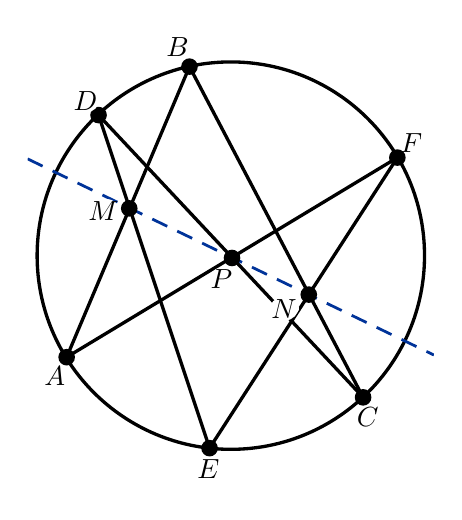
\begin{tikzpicture}[scale = 1.5]
    \clip(-1.72,-2) rectangle (1.72,1.93);
    \draw [line width=1.2pt] (0,0) circle (1.64cm);
    \draw [line width=1.2pt] (-1.39,-0.86)-- (-0.35,1.6);
    \draw [line width=1.2pt] (-0.35,1.6)-- (1.12,-1.2);
    \draw [line width=1.2pt] (1.12,-1.2)-- (-1.12,1.19);
    \draw [line width=1.2pt] (-1.12,1.19)-- (-0.18,-1.63);
    \draw [line width=1.2pt] (-0.18,-1.63)-- (1.41,0.83);
    \draw [line width=1pt,dash pattern=on 6pt off 4pt,color=qqttzz,domain=-1.72:1.72] plot(\x,{(-0.01-0.42*\x)/0.87});
    \draw [line width=1.2pt] (-1.39,-0.86)-- (1.41,0.83);
    \begin{scriptsize}
        \normalsize
        \fill [color=black] (-1.39,-0.86) circle (2.0pt);
        \draw[color=black] (-1.49,-1.02) node {$A$};
        \fill [color=black] (-0.35,1.6) circle (2.0pt);
        \draw[color=black] (-0.45,1.77) node {$B$};
        \fill [color=black] (1.12,-1.2) circle (2.0pt);
        \draw[color=black] (1.16,-1.37) node {$C$};
        \fill [color=black] (-1.12,1.19) circle (2.0pt);
        \draw[color=black] (-1.23,1.31) node[fill = white, rounded corners = 5pt, inner sep=0.8pt] {$D$};
        \fill [color=black] (-0.18,-1.63) circle (2.0pt);
        \draw[color=black] (-0.19,-1.81) node {$E$};
        \fill [color=black] (1.41,0.83) circle (2.0pt);
        \draw[color=black] (1.53,0.95) node[fill = white, rounded corners = 5pt, inner sep=0.8pt] {$F$};
        \fill [color=black] (-0.86,0.4) circle (2.0pt);
        \draw[color=black] (-1.08,0.38) node[fill = white, rounded corners = 5pt, inner sep=0.8pt] {$M$};
        \fill [color=black] (0.66,-0.33) circle (2.0pt);
        \draw[color=black] (0.45,-0.45) node[fill = white, rounded corners = 5pt, inner sep=0.8pt] {$N$};
        \fill [color=black] (0.01,-0.02) circle (2.0pt);
        \draw[color=black] (-0.08,-0.2) node[fill = white, rounded corners = 5pt, inner sep=0.8pt] {$P$};
    \end{scriptsize}
\end{tikzpicture}